% mnras_guide.tex
%
% MNRAS LaTeX user guide
%
% v3.0 released 22 May 2015
% (version numbers match those of mnras.cls)
%
% Copyright (C) Royal Astronomical Society 2015
% Authors:
% Keith T. Smith (Royal Astronomical Society)

% Change log
%
% v3.0   September 2013 - May 2015
%    First version: complete rewrite of the user guide
%    Basic structure taken from mnras_template.tex by the same author

%%%%%%%%%%%%%%%%%%%%%%%%%%%%%%%%%%%%%%%%%%%%%%%%%%
% Basic setup. Most papers should leave these options alone.
\documentclass[a4paper,fleqn,usenatbib]{mnras}

%%%%% AUTHORS - PLACE YOUR OWN PACKAGES HERE %%%%%

% MNRAS is set in Times font. If you don't have this installed (most LaTeX
% installations will be fine) or prefer the old Computer Modern fonts, comment
% out the following line
\usepackage{newtxtext,newtxmath}
% Depending on your LaTeX fonts installation, you might get better results with one of these:
%\usepackage{mathptmx}
%\usepackage{txfonts}

% Use vector fonts, so it zooms properly in on-screen viewing software
% Don't change these lines unless you know what you are doing
\usepackage[T1]{fontenc}
\usepackage{ae,aecompl}


%%%%% AUTHORS - PLACE YOUR OWN PACKAGES HERE %%%%%

% Only include extra packages if you really need them. Common packages are:
\usepackage{graphicx}	% Including figure files
\usepackage{amsmath}	% Advanced maths commands
\usepackage{amssymb}	% Extra maths symbols
\usepackage[english]{babel}
\usepackage{hyperref}

%%%%%%%%%%%%%%%%%%%%%%%%%%%%%%%%%%%%%%%%%%%%%%%%%%

%%%%%% AUTHORS - PLACE YOUR OWN MACROS HERE %%%%%%

% Please keep new commands to a minimum, and use \newcommand not \def to avoid
% overwriting existing commands. Example:
%\newcommand{\pcm}{\,cm$^{-2}$}	% per cm-squared
\newcommand{\kms}{\,km\,s$^{-1}$} % kilometres per second
\newcommand{\bibtex}{\textsc{Bib}\!\TeX} % bibtex. Not quite the correct typesetting, but close enough
\newcommand{\kb}{k_{\text{B}}}
\newcommand{\D}{\text{d}}
\newcommand{\x}{{\textit{\textbf{x}}}\,}
\newcommand{\y}{{\textit{\textbf{y}}}\,}
\newcommand{\n}{\hat{\textit{\textbf{n}}}}

%%%%%%%%%%%%%%%%%%%%%%%%%%%%%%%%%%%%%%%%%%%%%%%%%%


% Use vector fonts, so it zooms properly in on-screen viewing software
% Don't change these lines unless you know what you are doing
\usepackage[T1]{fontenc}
\usepackage{ae,aecompl}
\usepackage{bold-extra}
\usepackage{mathrsfs}

% MNRAS is set in Times font. If you don't have this installed (most LaTeX
% installations will be fine) or prefer the old Computer Modern fonts, comment
% out the following line
% \usepackage{newtxtext,newtxmath}
% Depending on your LaTeX fonts installation, you might get better results with one of these:
% \usepackage{mathptmx}
% \usepackage{txfonts}

%%%%%%%%%%%%%%%%%%% TITLE PAGE %%%%%%%%%%%%%%%%%%%

% Title of the paper, and the short title which is used in the headers.
% Keep the title short and informative.
\title[Magritte]{\textsc{Magritte}: a new multidimensional accelerated general-purpose radiative transfer code}

% The list of authors, and the short list which is used in the headers.
% If you need two or more lines of authors, add an extra line using \newauthor
\author[F. De Ceuster et al.]{
F. De Ceuster$^{1,2}$\thanks{Contact e-mail: \href{frederik.deceuster@kuleuven.be}{frederik.deceuster@kuleuven.be}},
J. Yates$^{1}$,
%J. Hetherington$^{3}$,
%P.A. Boyle$^{4}$,
L. Decin$^{2}$,
T.G. Bisbas$^{5,6}$,
S. Viti$^{1}$ and
M. Barlow$^{1}$
\\ \\
% List of institutions
$^{1}$Department of Physics and Astronomy, University College London, Gower Place, London, WC1E 6BT, UK \\
$^{2}$Department of Physics and Astronomy, Institute of Astronomy, KU Leuven, Celestijnenlaan 200D, 3001 Leuven, Belgium \\
%$^{3}$Research Software Development Group, University College London, Podium Building, 1 Eversholt Street, London, NW12DN, UK \\
%$^{4}$School of Physics and Astronomy, The University of Edinburgh, Edinburgh EH9 3FD, UK \\
$^{3}$Department of Astronomy and Physics, University of Florida, Gainesville, FL 32611, USA \\
$^{4}$Max-Planck-Institut f\"ur Extraterrestrische Physik, Giessenbachstrasse 1, D-85748 Garching, Germany}


% These dates will be filled out by the publisher
\date{Last updated 2011 May 22; in original form 2013 September 5}

% Enter the current year, for the copyright statements etc.
\pubyear{2018}

% Don't change these lines
\begin{document}
\label{firstpage}
\pagerange{\pageref{firstpage}--\pageref{lastpage}}
\maketitle

% Abstract of the paper
\begin{abstract}
	Radiative transfer is a key ingredient in understanding the dynamics, chemistry and energy balance of various astrophysical objects. Therefore it is essential in astrophysical modelling to properly account for all radiative processes and their interdependence. In this paper we present \textsc{Magritte}: a new multidimensional accelerated general-purpose radiative transfer code. \textsc{Magritte} is a grid-independent deterministic ray-tracing code that obtains the radiation field by solving the transfer equation along a fixed set of rays originating from each grid cell. It iteratively accounts for scattering and treats the full frequency space. Appended with a dedicated chemistry and thermal balance module \textsc{Magritte} can self-consitently calculate the temperature field, chemical abundances and level populations.

	\textsc{Magritte} is especially designed to have a well scaling performance on various computer architectures.   in stellar winds and perform synthetic observations. We will apply {\sc Margritte} by post-processing snapshots of hydrodynamical wind and bowshock simulations and will present its integration in self-consistent hydro-chemical AGB wind models.
\end{abstract}

% Select between one and six entries from the list of approved keywords.
% Don't make up new ones.
\begin{keywords}
radiative transfer, astrochemistry, methods: numerical
\end{keywords}

%%%%%%%%%%%%%%%%%%%%%%%%%%%%%%%%%%%%%%%%%%%%%%%%%%

%%%%%%%%%%%%%%%%% BODY OF PAPER %%%%%%%%%%%%%%%%%%


\section{Introduction}

Radiative transfer processes play a central role in the dynamics, the chemistry and the energy balance of all kinds of astrophysical objects. It provides a radiative pressure that can drive the dynamics, it affects the chemistry through various photoionization and photodissociation reactions, and it can very efficiently heat or cool very specific regions. Furthermore the radiative transfer determines how these objects appear in observations: which regions are visible in what part of the spectrum. Therefore it is essential in astrophysical modelling to properly account for all radiative processes and their interdependence. This however can be highly complicated by i) an intricate 3D geometrical structure shielding or exposing specific regions to radiation, ii) the scattering of radiation by dust or free electrons yielding additional non-trivial coupling between the geometry and the radiation field, and iii) the mixing in frequency space due to Doppler shifts caused by velocity gradients in the medium. The tight coupling between the radiative processes and the often very specialized but diverse dynamical and chemical models furthermore requires a modular solution method that can easily be integrated into various frameworks.

There are two main computational strategies used to solve radiative transfer problems. There are the probabilistic (Monte Carlo) codes e.g. \citep{SKIRT2011, RADMC2012, CMACIONIZE2018} and deterministic ray-tracing codes e.g. \citep{SPHRAY2011, Bisbas2012}. Nowadays most radiative transfer codes use probabilistic methods. They mimic the physical photon transport by propagating a number of photon packets through the medium. The main issue with this approach is that photon packets can get trapped in optically thick regions of the medium which can severely increase the computation time. Although many techniques have been devised to avoid the trapping of photon packets it remains a serious bottleneck for probabilistic codes. Deterministic ray-tracing codes do not suffer from photon trapping. They obtain the radiation field by (iteratively) solving the transfer equation along a number of fixed rays. The fixed (deterministic) computational scheme moreover leads to various opportunities for optimization (De Ceuster et al. \textit{in prep.}).

In this paper we present \textsc{Magritte}: a new multidimensional accelerated general-purpose radiative transfer code. \textsc{Magritte} is a deterministic ray-tracing code that is independent of the underlying grid structure. It can trace its rays only using the positions of the cell centers and the nearest neighbours lists. \textsc{Magritte} can iteratively account for anisotropic scattering by a range of dust species and free electrons. The methods are also flexible enough to be extended to scattering from aligned dust grains due to e.g. magnetic fields. The code treats the full frequency space including continuum radiation, and atomic and molecular lines. Appended with a dedicated chemistry and thermal balance module it can self-consitently calculate the temperature field, chemical abundances and level populations.

The development of the code started from the (open source) 3D astrochemistry code \textsc{3d-pdr}\footnote{\href{https://github.com/uclchem/3D-PDR}{github.com/uclchem/3D-PDR}} by \citet{Bisbas2012}. From there it was rewritten and restructured in a more object-oriented way in C++. Starting from an existing code allowed us to heavily test and benchmark the new structure used in \textsc{Magritte}. \textsc{3d-pdr} was made to self-consitently model the chemistry, some atomic and molecular lines and the thermal balance in phododissociation regions (PDRs). In \textsc{3d-pdr} the UV radiation field is obtained by direct integration, neglecting the diffusive radiation using the on-the-spot approximation \citep{Osterbrock1974}. When only considering external UV sources, this approximation is simple enough to allow for a self-consistent treatment of the UV radiation field and the UV photochemistry. The atomic and molecular line tranfer in \textsc{3d-pdr} is treated in the escape probability formalism using the large velocity gradient (LVG) or Sobolev approximation \citep{Sobolev1960, Castor1970, deJong1975, Poelman2005}. Using this approximation the line transfer can be used to calculate the radiative cooling fast enough to self-consitently calculate the temperature field by assuming thermal balance. Although the above assumptions are very useful and reasonable in some situations, they highly limit the applicability of the code. Another limitation to \textsc{3d-pdr} is the high memory cost due to the way in which the rays are stored. This limits the computational size of the models that can be run.

As a first step in the development of \textsc{Magritte} the old ray-tracer was rewritten to make use of the neighbours lists of the grid points. This improved its speed which allowed us to trace the rays on-the-fly thus avoiding the need to store them. This drastically reduces the memory cost. Afterwards the atomic and molecular line radiative transfer was replaced by an approximated lambda iteration (ALI) scheme. The new scheme does not make any assumptions on the velocity field and was extened to account for dust scattering. Finally the thermal balance module that self-consistently calculates the temperature field was made more robust. Thanks to the new grid-independent structure of \textsc{Magritte} we have a lot of flexibility in the way we use the grid. We can start the temperature calculations on a very coarse grid and use a slow but careful method to get an idea of the temperature field. Then we can interpolate this onto a more refined grid and recalculate the temperature using a faster method. Since we already had a reasonable idea of the temperature to start with, the faster method will still be stable. The flexibility to make the optimal trade-off between stability and performance is the guiding idea in the object-oriented design and structure of \textsc{Magritte}.

In this paper we mainly focus on the new physics that is implemented in \textsc{Magritte} and benchmark the accuracy of its output. In a forthcomming paper (De Ceuster et al. \textit{in prep.}) we will investigate further optimization and parallelization techniques that can be used to obtain optimal and scalable performance of \textsc{Magritte} on various computer architectures. Afterwards we plan to demonstrate the versatillity of the code by post-processing snapshots of hydrodynamical simulations of both stellar winds and composite galaxies. To demonstrate the modularity we plan to integrate it in \textsc{amrvac} \citep{Xia2018} to be used together with \textsc{krome} \citep{Grassi2014} in self-consistent radiative hydro-chemical AGB wind models.

This paper is organized as follows. In section \ref{Computational} we present the new computational scheme of \textsc{Magritte}. Section \ref{Benchmarks} describes the different benchmarks that were done to test the different modules and to compare its performance against \textsc{3d-pdr}. In Section \ref{Applications} we present some first novel applications. Finally our conclusions are discussed in Section \ref{Conclusions}.


\section{Computational Scheme}
\label{Computational}

Although \textsc{Magritte} is based on \textsc{3d-pdr} (Fortran), the whole code has been rewritten and restructured in C++. As input, \textsc{Magritte} takes an unstructured grid. For each grid cell one needs to specify the cell center, the total density and the local gas velocity. If known, one can also specify the nearest neighbours for each cell, otherwise these are calculated by \textsc{Magritte}. Except for the neighbours no other attributes of the grid (e.g. cell edges or faces) are needed. The code does not dependent on the underlying structure (i.e. the tessellation) of the grid. This enables us to easily handle various types of input, from AMR-grids to Voronoi grids as well as SPH-particle data\footnote{We are aware that specifying a certain type of grid (e.g. Voronoi) can further improve the performance in terms of speed. In future versions, when \textsc{Magritte} is used in combination with certain other codes, we will optimize for certain grids.}.


\begin{figure}
	\centering
	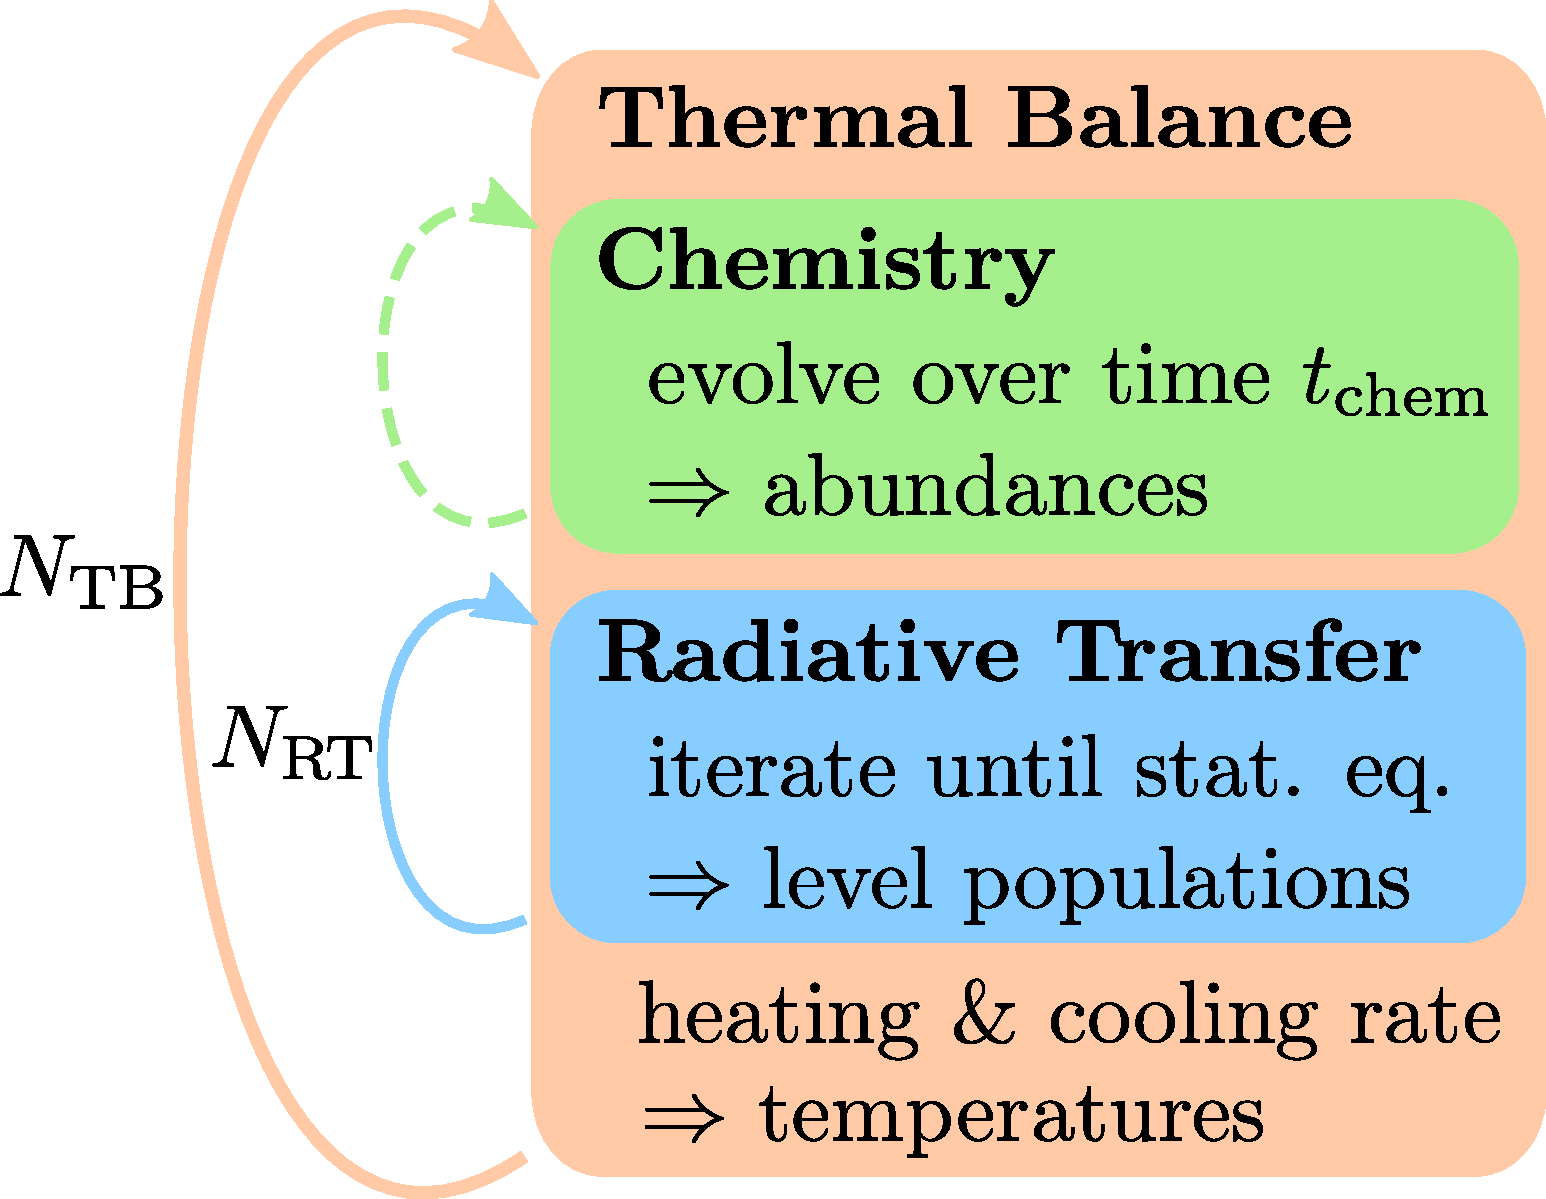
\includegraphics[width=.9\columnwidth]{figures/scheme.pdf}
  \caption{Iteration schemes of the Magritte workflow, different boxes represent the different modules.}
  \label{scheme}
\end{figure}


\subsection{Ray-tracing}

\textsc{Magritte} is a deterministic ray-tracing code. The radiation field is determined by solving the radiative transfer equation on a fixed set of rays (i.e. straight lines) originating from each cell center. The mean intensity in a cell is then obtained by averaging over the radiation along the different rays. The direction of a ray is determined by the \textsc{HEALPix}\footnote{\href{http://healpix.sourceforge.net}{healpix.sourceforge.net}} discretization of the sphere \citep{Gorski2005}. Given a level of refinement $\ell$, it discretizes the unit sphere in $N_{\text{rays}}=12 \times 4^{\ell}$ uniformly distributed pixels of equal area. For each pixel there is an associated unit vector pointing from the origin of the unit sphere to the pixel center. Our rays are thus defined as the straight lines originating from the cell centers in the directions of these unit vectors.

\subsubsection{Constructing the rays}

In order to solve the transfer equation along a certain ray, we need to know the emissivity and opacity of the cells that are encountered along that ray. Furthermore we need to know the path length of a ray through a certain cell. This is slightly complicated since the only geometrical information we required from the cells is the location of their cell center and their nearest neighbours. The solution as implemented in \textsc{Magritte} is to walk along the ray and project nearest cell centers onto the ray. Consider a ray originating from a cell, say $o$ (see figure \ref{next_cell}). Clearly the cell $o$ itself should lie on the ray. The next cell to be projected on the ray is the neighbour of $o$ that lies closest to the ray. We will call this cell $p_{1}$. Now the next cell to be projected is the neighbour of $p_{1}$ that lies closest to the ray and that is further away from $o$ than $p_{1}$. The last condition is there to ensure that one proceeds along the ray towards the boundary. This process is repeated untill the boundary of the gird is reached.

The above algorithm constructs the ray from a given cell outward to the boundary. However it is also useful to be able to do the opposite and construct a ray from the boundary inward towards a certain cell. We will refer to this cell for the moment as the origin. To do this one needs to know the end point of each ray, i.e. the final cell of the boundary that will be projected on the ray. These are calculated and stored in the setup of \textsc{Magritte}. Once the endpoints are known the above algorithm can be used to walk along the ray from the boundary to the origin of the ray. The only difference is that one should pick the next cell closest to the ray and that is closer to the origin instead off further away. The last condition is again there to ensure that one recedes along the ray back to the origin.

\begin{figure}
	\centering
	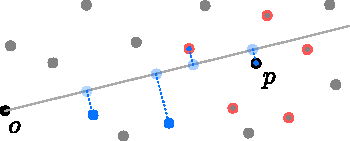
\includegraphics[width=.9\columnwidth]{figures/next_cell.pdf}
  \caption{Sketch of the algorithm that chooses which cells to project on a ray. All cells are represented by their cell centers. The ray originates from the black cell (denoted $o$). The blue cells are already projected onto the ray. The blue cell with the black border (denoted $p$) is the last cell that was projected. The neighbours of $p$ are indicated with red borders. The next cell to be projected is the neighbor of $p$ with a projection on the ray further than the projection of $p$, that lies closest to the ray.}
  \label{next_cell}
\end{figure}


\subsubsection{Ray-tracing in \textsc{Magritte} vs. \textsc{3d-pdr}}

In \textsc{3d-pdr} the projections of all cells on the rays for each cell are calculated during setup (using a different algorithm) and kept in memory. This is a huge amount amount of data to be stored which scales as $N_{\text{cells}} \times N_{\text{cells}} \times N_{\text{rays}}$. This quickly leads to memory issues, severely limiting the grid size of the simulations that can be run. In \textsc{Magritte} we only store the projections of the cells on the rays for one cell at the time. This reduces the scaling of the memory cost to $N_{\text{cells}} \times N_{\text{rays}}$ which allows us to run simulations with much larger grids on the same machine.



\subsection{Chemistry}

The chemistry module is largly based on the chemical gas-grain code \textsc{uclchem} \citep{Holdship2017}. We opted to rewrite the needed parts of the code in our framework rather than using it to facilitate future extentions. In this module \textsc{Magritte} can determine the relative abundances of a limited number of atomic and molecular species at each cell. This is done by solving the time-dependent chemistry of a self-contained network of formation and destruction reactions. The chemical network is a subset of the most recent UMIST data base of reaction rates \citep{Woodall2007}, consisting of 320 reactions between 33 species (including electrons), and includes photoionization and photodissociation reactions in addition to the standard gas-phase chemistry.




\subsection{Level populations}
Given the chemical abundances, \textsc{Magritte} can calculate the level populations for a subsset of the chemical species. The evolution of the population $n_{i}$ of the level $i$ of a species with $N$ levels in the comoving frame is given by the transition rate to that level minus the transition rate form that level
\begin{equation}
	\frac{\partial n_{i}(\x)}{\partial t} \ = \
	\sum_{j=1}^{N} n_{j}(\x) R_{ji}(\x) \ - \ n_{i}(\x) \sum_{j=1}^{N} R_{ij}(\x) .
\label{levelpop}
\end{equation}
The transition rates in terms of Einstein coefficients read
\begin{equation}
	R_{ij}(\x) \ = \ A_{ij} \ + \ 4\pi B_{ij}  J_{ij}(\x) \ + \ C_{ij}(\x),
\end{equation}
which account for the spontanious ($A_{ij}$), stimulated ($B_{ij}$) and collisional ($C_{ij}(\x)$) transitions. Note that $A_{ij}=0$ for $i \leq j$ and that the collisional Einstein coefficients have a position dependence because they depend on the local gas temperature. In our simulations we used the line data from the Leiden Atomic and Molecular Database \citep[LAMDA,][]{Schoier2005}. $J_{ij}(\x)$ is the local mean intensity in the spectral range of the transition $i \leftrightarrow j$. In general the intensity itself depends on the level populations. Therefore one needs to solve iteratively for the level populations, each time using the values of the previous iteration to compute the mean intensity. In \textsc{Magritte} this is done assuming local statistical equilibrium, i.e. $\partial n_{i}(\x)/\partial t = 0$.



\subsubsection{Radiative transfer}

The local mean intensity $J_{ij}(\x)$ in the spectral range of a transition $i \leftrightarrow j$ is the monochromatic specific intensity $I_{\nu}(\x, \n)$ averaged over all directions and intergrated over the whole spectrum weighted by the local line profile $\phi_{\nu}^{ij}(\x)$,
\begin{equation}
	J_{ij}(\x) \ = \ \oint \frac{\D\Omega}{4\pi} \int_{0}^{\infty} \D\nu \ \phi_{\nu}^{ij}(\x) \ I_{\nu}(\x, \n).
\end{equation}
To obtain the average over all directions, \textsc{Magritte} computes the intensity along all rays and averages over the rays. To obtain the weighted integral over the spectrum \textsc{Magritte} computes the intensity for certain frequencies given by a quadrature scheme.

In the simulations presented in this paper we always assumed Gaussian profile functions\footnote{\textsc{Magritte} can cope with any user defined profile function as long as the appropriate roots and weights for the quadrature are also provided by the user.} such that the integrals over the spectrum can be done using a Gauss-Hermitte quadrature. A Gaussian profile function in the comoving frame reads,
\begin{equation}
	\phi_{\nu}^{ij}(\x) \ = \ \frac{1}{\sqrt{\pi}\delta\nu_{ij}} \ \exp \left(-\left(\frac{\nu-\nu_{ij}} {\delta\nu_{ij}}\right)^{2}\right),
\end{equation}
where the width $\delta\nu$ of the profile is due to the Doppler shifts caused by motions of the atoms and molecules in a cell,
\begin{equation}
	\left(\frac{\delta\nu_{ij}}{\nu_{ij}}\right)^{2} \ = \ \frac{2 \kb T(\x)}{\pi mc^{2}} \ + \ \left(\frac{v_{\text{turb.}}}{c}\right)^{2}.
\end{equation}
The first term is due to thermal motions (along the line of sight) and the second is due to the turbulent motion.

To find in each direction ($\n$) the monochromatic specific intensity, \textsc{Magritte} solves the radiative transfer equation in the comoving frame along each ray.
\begin{equation}
	\n \cdot \nabla I_{\nu}(\x,\n) \ = \ \eta_{\nu}(\x,\n) \ - \ \chi_{\nu}(\x) \ I_{\nu}(\x,\n).
\label{transfer}
\end{equation}
The emissivity $\eta_{\nu}(\x,\n)$ and opacity $\chi_{\nu}(\x)$ can be split into a line, a continuum and a scattering term,
\begin{equation}
\begin{split}
		\eta_{\nu}(\x,\n) \ &= \ \eta^{ij}_{\nu}(\x) \ + \ \eta^{\text{con.}}_{\nu}(\x) \ + \ \eta^{\,\text{sca.}}_{\nu}(\x,\n) \\
		\chi_{\nu}(\x)   \ &= \ \chi^{ij}_{\nu}(\x) \ + \ \chi^{\text{con.}}_{\nu}(\x) \ + \ \chi^{\,\text{sca.}}_{\nu}(\x).
\end{split}
\label{scattering}
\end{equation}
The line emissivity and opacity are caused by the transitions between the level populations and can be expressed in terms of the Einstein coefficients,
\begin{equation}
\begin{split}
\eta^{ij}_{\nu}(\x) \ &= \ \frac{h\nu}{4\pi} \ A_{ij} \ n_{i}(\x) \ \phi^{ij}_{\nu}(\x), \\
\chi^{ij}_{\nu}(\x) \ &= \ \frac{h\nu}{4\pi} \ \Big( B_{ji} \ n_{j}(\x) \ - \ B_{ij} \ n_{i}(\x) \Big) \ \phi^{ij}_{\nu}(\x).
\end{split}
\end{equation}
The continuum terms are due to dust. \textsc{Magritte} contains one dust species with a certain dust temperature $T_{\text{dust}}(\x)$. The cosmic microwave background (CMB) is treated as a boundary condition.



\textsc{Magritte} solves the monochromatic transfer equation in Feautrier form \citep{Feautrier1964} using the improved numerical scheme suggested by \citet{Rybicki1991}. In this method the transfer equation is rewritten as a second-order differential equation
\begin{equation}
	u_{\nu}(\x, \n) \ = \ \frac{1}{2}\Big( I_{\nu}(\x, \n) \ + \ I_{\nu}(\x, -\n) \Big)
\end{equation}

\begin{equation}
	\frac{\D^{2}u_{\nu}(\x, \n)}{\D\tau_{\nu}^{2}} \ = \ u_{\nu}(\x, \n) \ - \ S_{\nu}^{\,\text{eff.}}(\x, \n)
\end{equation}



In \textsc{3d-pdr} the radiative transfer is solved in the escape probability formalism and applying the large velocity gradient (LVG) or Sobolev approximation \citep{Sobolev1960, Castor1970, deJong1975, Poelman2005}. This is still an option in Magritte. The mean intensity is given by








\subsubsection{Accelerated Lambda Iterations (ALI)}

The convergence of the level populations can be notoriously slow. In order to account for this, many acceleration methods have been devised over the years. In \textsc{Magritte} we used an approximated lambda operator scheme introduced by \citet{Rybicki1991}, complemented by the Ng-acceleration method \citep{Ng1974}.

The approximated lambda operator scheme of \citeauthor{Rybicki1991} reoders the transition coefficients as
\begin{equation}
	R_{ij}(\x) \ = \ A_{ij} \left(1-\Lambda^{\ast}_{ij}(\x)\right) \ + \ B_{ij}  J^{\,\text{eff.}}_{ij}(\x) \ + \ C_{ij}(\x),
\label{RybickiHummer}
\end{equation}
where the approximated lambda operator $\Lambda^{\ast}_{ij}(\x)$ and the resulting effective mean intensity $J^{\,\text{eff.}}_{ij}(\x)$ are given by
\begin{equation}
\begin{split}
	\Lambda^{\ast}_{ij}(\x)    \ &= \ \\
	J^{\,\text{eff.}}_{ij}(\x) \ &= \ \\
\end{split}
\end{equation}

In the Ng-acceleration method \citep{Ng1974} a new educated guess for the level populaions is made based on the level populations in previous iterations.

The combination of both acceleration schemes yields a significant speed-up in the convergence of the level populations. In the Sobolev case the number of iterations over the level populations is reduced to $\mathcal{N}_{\text{pop}} \approx 3$, which is an improvment by a factor 10 (?), see Appendix \ref{Sobolev}. Note that the Ng-acceleration is redundant in this case since there are not enough iterations. Since this is such a simple way to obtain a such a drastic improvment in performance it was also implemented in a new update to \textsc{3D-pdr}\footnote{\href{https://github.com/uclchem/3D-PDR}{github.com/uclchem/3D-PDR}}.



In the general case theIn the general case the
\subsection{Thermal balance}

\textsc{Magritte} can iteratively determine the gas temperature, consistent with the chemical and radiative state, by demanding local thermal balance, i.e. equal heating and cooling rates in each cell. This assumes that the dynamical timescale of the system is large enough to be negligible. This is for instance the case in simulations of photodissociation regions (PDRs), see (citations!).

The temperature is iteratively calculated using the following scheme: Assuming a certain temperature field, the chemical abundances and level populations are calculated using their respective modules. These can be used to calculate the heating and cooling rates in each cell. Then a new guess can be made

The modular design of the code and the relatively simple structure of our cells allows us to do the




\section{Benchmarks}
\label{Benchmarks}

\subsection{Ray-tracing}

Angular resolution tests

\subsection{Line radiative transfer}

In order to test \textsc{Magritte}'s new radiative transfer module, it was compared against the results of the \citet{VanZadelhoff2002} benchmark.


\subsection{Dust scattering}


\subsection{{\sc Magritte} vs. {\sc 3d-pdr}}


\subsection{{\sc Magritte} vs. {\sc Lime}}
In order to test \textsc{Magritte}'s new radiative transfer module, it was benchmarked against \textsc{Lime} \citep{Brinch2010}.



\section{Applications}
\label{Applications}
The modular character of Magritte allows it to be easily used in various astrophysical simulations.




\section{Conclusions}
\label{Conclusions}
We have presented Magritte: a new multidimensional accelerated general-purpose radiative transfer code.

\bigskip

The source code for Magritte and its separate modules will eventually be made freely available on \href{https://github.com/Magritte-code}{github.com/Magritte-code}. In the mean time various parts can be made available upon request.




\section*{Acknowledgements}
The authors would like to thank C.P. Dullemond and C. Brinch for helpful and encouraging discussions.

FDC is supported by the EPSRC iCASE studentship programme, Intel Corporation and Cray Inc.




\bibliography{library}
\bibliographystyle{mnras}




\appendix




\section{ALI in the escape probability formalism}
\label{Sobolev}

In \textsc{3d-pdr} the radiative transfer is solved in the escape probability formalism and applying the large velocity gradient (LVG) or Sobolev approximation \citep{Sobolev1960, Castor1970, deJong1975, Poelman2005}. In this approximate formalism the mean intensity in the spectral range of a transition $i \leftrightarrow j$ is given by
\begin{equation}
J_{ij}(\x) \ = \ \left(1-\beta_{ij}(\x)\right) S^{\,\text{line}}_{ij}(\x) \ + \ \beta_{ij}(\x) J^{\,\text{con.}}_{ij}(\x)
\end{equation}
where the escape probability $\beta_{ij}(\x)$ is cumputed as,
\begin{equation}
	\beta_{ij}(\x) \ = \ \oint \frac{\D \Omega}{4\pi} \ \frac{1-e^{-\tau_{ij}(\x,\n)}}{\tau_{ij}(\x,\n)}
\end{equation}
in terms of the line optical depth
\begin{equation}
	\tau_{ij}(\x,\n) \ = \ \int_{0}^{\infty} \D s \ \chi_{ij}(\x+s\n)
\end{equation}
The approximated lambda operator and associated effective mean intensity, as defiined by \citet{Rybicki1991} is in this case simply given by
\begin{equation}
\begin{split}
	\Lambda^{\ast}_{ij}(\x) \ &= \ 1 \ - \ \beta_{ij}(\x) \\
	J^{\,\text{eff.}}_{ij}(\x) \ &= \ \beta_{ij}(\x) \ J^{\,\text{con.}}_{ij}(\x).
\end{split}
\end{equation}
Substituted in equation (\ref{RybickiHummer}) this yiels
\begin{equation}
	R_{ij}(\x) \ = \  \beta_{ij}(\x) \left( A_{ij} \ + \ B_{ij} J^{\,\text{con.}}_{ij}(\x) \right) \ + \ C_{ij}(\x),
\end{equation}
This simple reorderig of terms in the transition rates yields a significant improvment in the convergence of the level populations. The number of iterations is reduced to $\mathcal{N}_{\text{pop}} \approx 3$, which is an improvment by a factor 10 (?). Since this simple change leads to such a major performance improvment it will also be included in \textsc{3d-pdr}.




\section{Scattering in the Feautrier formalism}
\label{Scattering}

The radiative transfer equation relates the change in specific monochromatic intensity $I_{\nu}(\x,\n)$ along a ray in direction $\n$ to the local emissivity $\eta_{\nu}(\x)$ and opacity $\chi_{\nu}(\x)$. For local radiative processes one can assume that both the emissivity $\eta_{\nu}(\x)$ and the opacity $\chi_{\nu}(\x)$ are isotropic, i.e. independent of the direction $\n$. When considering scattering \citep[see e.g.][]{Chandrasekhar1960,Steinacker2013} there is an extra direction-dependent emmisivity term in the transfer equation
\begin{equation}
\begin{split}
	\n \cdot \nabla I_{\nu}(\x,\n) \ = & \ \eta_{\nu}(\x) \ - \ \chi_{\nu}(\x) \ I_{\nu}(\x,\n) \\ & \ + \ \oint \D\Omega \ \Psi_{\nu}(\x, \n \, ,\n') \ I_{\nu}(\x,\n').
\label{transfer}
\end{split}
\end{equation}
where $\Psi(\x, \n \, ,\n')$ is the scattering redistribution function which gives the probability of an incoming photon along direction $\n'$ to be absorbed and then scattered in direction $\n$. To solve the transfer equation we can proceed, as suggested by \citet{Feautrier1964}, by defining
\begin{equation}
\begin{split}
		u_{\nu}(\n) \ &= \ \frac{1}{2}\Big( I_{\nu}(\n) \ + \ I_{\nu}(-\n) \Big), \\
		v_{\nu}(\n) \ &= \ \frac{1}{2}\Big( I_{\nu}(\n) \ - \ I_{\nu}(-\n) \Big).
\end{split}
\end{equation}
Adding and subtracting the transfer equation (\ref{transfer}) for $\n$ and $-\n$ yields a coupled set of equation for $u_{\nu}(\n)$ and $v_{\nu}(\n)$.
\begin{equation}
\begin{split}
		\n \cdot \nabla u_{\nu}(\n) \ = \ & \frac{1}{2}\Big( \eta_{\nu}(\n)
		\ - \ \eta_{\nu}(-\n) \Big) \ - \ \chi_{\nu} \ v_{\nu}(\n) \\
		\n \cdot \nabla v_{\nu}(\n) \ = \ & \frac{1}{2}\Big( \eta_{\nu}(\n)
		\ + \ \eta_{\nu}(-\n) \Big) \ - \ \chi_{\nu} \ u_{\nu}(\n)
\end{split}
\label{uv}
\end{equation}
Defining the monochromatic optical depth as usual
\begin{equation}
	\D\tau_{\nu} \ = \ \chi_{\nu} \ \n \cdot \D \x,
\end{equation}
equation (\ref{uv}) can be solved for $u_{\nu}(\x,\n)$.
\begin{equation}
\begin{split}
	\frac{\D^{2} u_{\nu}(\n)}{\D \tau_{\nu}^{2}} \ = & \ u_{\nu}(\n) \ - \ \frac{ \eta^{\,\text{eff.}}_{\nu}(\n) \ + \ \eta^{\,\text{eff.}}_{\nu}(-\n) }{ 2\chi^{\,\text{eff.}}_{\nu} } \\
	\ &+ \ \frac{\D}{\D\tau_{\nu}} \left( \frac{ \eta^{\,\text{eff.}}_{\nu}(\n) \ - \ \eta^{\,\text{eff.}}_{\nu}(-\n) }{ 2\chi^{\,\text{eff.}}_{\nu} } \right)
\end{split}
\end{equation}
Substituting the effective emissivities obtained in equation (\ref{etasca}) gives the Feautrier equation including scattering,
\begin{equation}
\begin{split}
	\frac{\D^{2} u_{\nu}(\n)}{\D \tau_{\nu}^{2}} \ = \ u_{\nu}(\n) - S^{\,\text{eff.}}_{\nu}(\n),
\end{split}
\end{equation}
where the effective source function is defined as
\begin{equation}
\begin{split}
	S^{\,\text{eff.}}_{\nu}(\n) \ = & \ \frac{\eta_{\nu}}{\chi^{\,\text{eff.}}_{\nu}} \ - \ \frac{  \chi^{\,\text{sca.}}_{\nu}}{ \chi^{\,\text{eff.}}_{\nu}} \oint \D\Omega \ \Phi(\n\cdot\n') \ u_{\nu}(\n') \\
	& \ + \ \frac{\D}{\D\tau_{\nu}}  \left( \frac{  \chi^{\,\text{sca.}}_{\nu}}{ \chi^{\,\text{eff.}}_{\nu}} \oint \D\Omega \ \Phi(\n\cdot\n') \ v_{\nu}(\n') \right).
\end{split}
\end{equation}
Solving the full Feautrier equation with scattering is intractable because of the $u_{\nu}(\n)$ and $v_{\nu}(\n)$ dependence in $S^{\,\text{eff.}}_{\nu}(\n)$. However, since we already have to solve the transfer iteratively because of the level populations, we can replace the effective source function with the one calculated in the previous iteration.

When discretizing the integrals over the directions in the transfer equation it is clearely beneficial to move the forward scattering term from the emissivity to the opacity,
\begin{equation}
\begin{split}
		\eta^{\,\text{eff.}}_{\nu}(\n) \ &= \ \eta_{\nu} \ + \ \eta^{\,\text{sca.}}_{\nu}(\n) \\
		\chi^{\,\text{eff.}}_{\nu}     \ &= \ \chi_{\nu} \ + \ \Big(1 - \Phi(\n\cdot\n)\Big)\chi^{\,\text{sca.}}_{\nu}
\end{split}
\label{scattering}
\end{equation}
such that now the emissivity reads
\begin{equation}
	\eta^{\,\text{sca.}}_{\nu}(\n) \ = \ \chi^{\,\text{sca.}}_{\nu} \sum_{\n' \neq \n} \ \Phi(\n\cdot\n') \ I_{\nu}(\n').
\label{etasca}
\end{equation}
Since the scattering phase function is strongly peaked around $\n' = \n$ this reduces the contributions of the scattering terms in the effective source function. This will improve the convergence of the iterations over the level populations.


%%%%%%%%%%%%%%%%%%%%%%%%%%%%%%%%%%%%%%%%%%%%%%%%%%


% Don't change these lines
\bsp	% typesetting comment
\label{lastpage}
\end{document}
